%% Adaptive UKF USBL positioning — manuscript (IEEE journal format)
%% Living document. Lives at project root; edited in place across folders.
%% Source lineage: folder 105 tightened MD (content) + folder 96 refs (bib).
%% Format convention (2026-07-12, user directive): LaTeX / IEEEtran only. No Word/DOCX.
\documentclass[journal]{IEEEtran}

\usepackage{amsmath,amssymb}
\usepackage{graphicx}
\usepackage{booktabs}
\usepackage{tabularx}
\usepackage{array}
\usepackage{url}
\usepackage[hidelinks]{hyperref}

\graphicspath{{figures/}}

% Left-ragged wrapping column for wide content tables
\newcolumntype{L}{>{\raggedright\arraybackslash}X}

\begin{document}

\title{Carrier-Agile Whitening of Coherent Multipath DOA Bias in Static Shallow-Water USBL Tracking}

\author{Author names and affiliations to be completed before submission.%
\thanks{Manuscript draft. This LaTeX source is the living manuscript of the project
(IEEEtran journal format). Content is frozen from the validated results; only formatting
is migrated to LaTeX.}}

\markboth{Manuscript draft, IEEEtran journal format}%
{Carrier-Agile Whitening of Coherent Multipath DOA Bias in Static Shallow-Water USBL Tracking}

\maketitle

\begin{abstract}
Frequency diversity is established in radar, sonar, and underwater positioning, but its role
in compact shallow-water USBL tracking remains mechanism-dependent. This paper asks whether
ping-to-ping carrier agility can reduce the post-gating coherent multipath direction-of-arrival
(DOA) bias that limits long-range localization. We study this question in a TOA/TDOA/DOA
unscented Kalman filter (UKF) framework. First, we characterize a long-range elevation-bias
floor that persists after direct-path gating and is amplified by the small aperture of an
eight-sensor USBL array. We then show that the bias contains a carrier-locked component: under
fixed-frequency transmission, direct and in-gate surface-reflected paths keep a nearly constant
interference phase, whereas carrier agility rotates this phase and whitens part of the residual.
With the carrier schedule fixed before validation, independent 600~m static experiments reduced
settled RMSE from 13.01~m to 8.87~m ($-32\%$, $p=0.0008$). The same mechanism whitened
moving-target residuals, but did not yield reliable pooled RMSE improvement, revealing a
boundary caused by motion-induced self-whitening and tail risk. Slow-drift validation supported
continuous quasi-static use only up to 0.005~m/s. The novelty is therefore not frequency hopping
itself, but the mechanism, validation, and boundary of carrier-agile whitening for coherent
multipath DOA bias in shallow-water USBL tracking.
\end{abstract}

\begin{IEEEkeywords}
USBL localization, underwater acoustic positioning, carrier agility, coherent multipath,
direction-of-arrival bias, TOA/TDOA/DOA fusion, unscented Kalman filter, shallow water,
frequency diversity, sensor fusion.
\end{IEEEkeywords}

\section{Introduction}
\IEEEPARstart{U}{nderwater} localization is a central function for autonomous underwater
vehicles, moored instruments, docking systems, and compact surface or subsea platforms.
Ultra-short baseline (USBL) systems are attractive because they can infer bearing from a compact
hydrophone array while also using acoustic time-of-arrival information. However, compact aperture
is also the source of a difficult accuracy limitation: at long range, small angular errors
produce large position errors.

This work began from a conventional tracking question: can TOA, TDOA, and DOA measurements be
fused with a Kalman-family estimator to improve 3-D underwater localization? A UKF-based tracker
is indeed a useful backbone, particularly because the observation model is nonlinear and EKF
linearization becomes fragile at longer range. Yet the dominant limitation observed in the
present shallow-water signal simulations was not simply a filter problem. Even after direct-path
time gating and adaptive measurement covariance routing, a systematic elevation component
remained.

Multipath mitigation, USBL calibration, and frequency-diverse acoustic signaling are all mature
topics. Radar literature has long used frequency agility to decorrelate glint-like angular
errors~\cite{Loomis1974FrequencyAgilityGlint}, and underwater positioning literature includes
frequency-hopped acoustic modem USBL, Costas-based USBL design, acoustic frequency-comb
approaches, and other frequency-diversity methods~\cite{Beaujean2007FrequencyHoppedUSBL,
Nhat2022CostasUSBL, Qian2025FrequencyCombIUSBL}. Table~\ref{tab:priorart} distinguishes these
prior families from the present work. The contribution here is not the first use of frequency
hopping. The gap is narrower: the post-gating DOA residual in a compact shallow-water USBL array
can contain a carrier-locked coherent multipath component, and a transmit-side carrier schedule
can whiten this residual before it is fused by a TOA/TDOA/DOA-UKF tracking loop.

We propose ping-to-ping carrier agility as an observation design rather than as a new
receiver-side estimator. The receiver extracts the same observation vector: one absolute
TOA-derived range, seven reference TDOA-derived range differences, and two DOA angles. The UKF
fusion pipeline is kept fixed. What changes is the temporal structure of the residual entering
the filter.

The paper makes four contributions. First, it characterizes a post-gating long-range DOA bias
floor in compact shallow-water USBL tracking. Second, it identifies a carrier-sensitive coherent
mechanism that explains why the residual changes with carrier frequency. Third, it validates a
frozen 30--34~kHz ping-to-ping carrier schedule on independent 600~m static-target trials.
Fourth, it quantifies the boundary: moving targets show strong residual whitening but not
reliable pooled RMSE improvement, and a slow-drift sweep supports continuous quasi-static use
only up to 0.005~m/s under the current protocol.

\begin{table*}[!t]
\centering
\caption{Positioning of the present work relative to related frequency-diverse and USBL
localization literature. The distinction claimed here is not the first use of frequency hopping
in USBL, but the identification and validation of carrier-agile whitening for post-gating
coherent multipath DOA bias in a TOA/TDOA/DOA-UKF tracking loop.}
\label{tab:priorart}
\footnotesize
\begin{tabularx}{\textwidth}{L c c L c c L}
\toprule
Literature family & Freq.\ diversity? & USBL pos.? & Main purpose in prior work &
Post-gating DOA-bias whitening? & UKF boundary quantified? & How this paper differs \\
\midrule
Radar frequency agility / glint reduction~\cite{Loomis1974FrequencyAgilityGlint} & Yes & No &
Decorrelate radar angular/glint tracking errors & Partly analogous, not underwater USBL
multipath & No & Cited as closest physical analogy; we narrow the claim to shallow-water USBL and
surface-reflection coherent DOA residuals. \\
Frequency-hopped acoustic modem USBL~\cite{Beaujean2007FrequencyHoppedUSBL} & Yes & Yes &
Frequency-hopped acoustic modem sequences for positioning & Not established as target mechanism &
No & Prior existence prevents a ``first FH USBL'' claim; our contribution is the residual-whitening
mechanism and validation boundary. \\
Costas / hopped USBL shallow-water designs~\cite{Nhat2022CostasUSBL} & Yes & Yes & Improve
correlation, time-delay, or navigation precision & Not the stated mechanism & No & Related waveform
diversity exists, but does not isolate carrier-locked post-gating DOA bias entering a UKF tracker. \\
Acoustic frequency-comb / iUSBL approaches~\cite{Qian2025FrequencyCombIUSBL} & Yes & Often iUSBL &
Comb/frequency-diverse signals for positioning or processing & Not the stated mechanism & No &
Frequency diversity is used, but the system role and residual mechanism differ. \\
USBL calibration / installation-error correction & Usually no & Yes & Estimate mounting,
alignment, or calibration errors & No & No & Calibration removes static system errors; here the
residual remains tied to carrier-sensitive propagation after gating. \\
\textbf{Present work} & Yes (ping-to-ping) & Yes (8-sensor) & Change the temporal structure of the
residual entering TOA/TDOA/DOA-UKF fusion & \textbf{Yes} & \textbf{Yes} & Static 600~m improvement
validated; moving/quasi-static boundary explicitly reported, including negative results. \\
\bottomrule
\end{tabularx}
\end{table*}

\section{System and Signal Model}
We consider a compact eight-sensor USBL array in a shallow-water acoustic environment. Let the
source position at ping $k$ be $p_k=[x_k,y_k,z_k]^{T}$, and let the $i$-th receiver element
position be $s_i$, $i=0,\ldots,7$. The array center is
\begin{equation}
\bar{s}=\frac{1}{8}\sum_{i=0}^{7}s_i,
\end{equation}
and the geometric source-to-sensor range is
\begin{equation}
\rho_{i,k}=\|p_k-s_i\|_2 .
\end{equation}
The signal-derived observation vector is
\begin{equation}
z_k =
\begin{bmatrix}
r_{0,k} & \Delta r_{1,k} & \cdots & \Delta r_{7,k} & \alpha_k & \epsilon_k
\end{bmatrix}^{T},
\end{equation}
where $r_{0,k}$ is the reference-sensor TOA-derived range, $\Delta r_{i,k}$ is the TDOA-derived
range difference, and $\alpha_k$, $\epsilon_k$ are azimuth and elevation. The ideal range and
TDOA terms are
\begin{equation}
r_{0,k}=\rho_{0,k},\quad \Delta r_{i,k}=\rho_{i,k}-\rho_{0,k},\quad i=1,\ldots,7.
\end{equation}
With $d_k=p_k-\bar{s}$, the ideal DOA components are
\begin{align}
\alpha_k &=\operatorname{atan2}(d_{k,y},d_{k,x}),\\
\epsilon_k &=\operatorname{atan2}\!\left(d_{k,z},\sqrt{d_{k,x}^2+d_{k,y}^2}\right).
\end{align}
The UKF state is
\begin{equation}
x_k=[p_k^{T},u_k^{T}]^{T}
=\begin{bmatrix} x_k & y_k & z_k & v_{x,k} & v_{y,k} & v_{z,k} \end{bmatrix}^{T},
\end{equation}
and a constant-velocity transition is used:
\begin{equation}
x_{k+1}=Fx_k+w_k,\quad
F=\begin{bmatrix} I_3 & \Delta t\, I_3 \\ 0_3 & I_3 \end{bmatrix}.
\end{equation}
The measurement model is
\begin{equation}
z_k=h(x_k)+v_k,
\end{equation}
where $v_k$ includes timing, TDOA, DOA, and coherent multipath residual components. A conditional
adaptive-$R$ wrapper changes the measurement covariance according to a signal-consistency
indicator $g_k$, defined as the GCC/SRP DOA disagreement in degrees. The wrapper operates in two
stages. First, a graded scale is computed as
\begin{equation}
s_k=\min\!\left(100,\;1+\left(\frac{g_k}{2}\right)^{2}\right).
\end{equation}
The scale is applied to the DOA block of $R_k$ when $g_k\le\tau$, and to the TDOA block when
$g_k>\tau$, with $\tau=5^{\circ}$. This routes uncertainty toward the observation block that is
less consistent with the current signal evidence. Second, each measurement block is independently
checked by a normalized innovation squared (NIS) test:
\begin{equation}
R_k^{(b)}\leftarrow
R_k^{(b)}\cdot\min\!\left(100,\;\max\!\left(1,\;\frac{\mathrm{NIS}_k^{(b)}}{\chi^2_{0.99}(d_b)}\right)\right),
\end{equation}
where $b$ denotes the TOA-range, TDOA, and DOA blocks with degrees of freedom $d_b=1,7,2$,
respectively. The corresponding $\chi^2_{0.99}$ thresholds are 6.63, 18.48, and 9.21. This
adaptive-$R$ rule is used as the tracking backbone. The proposed contribution is not a new UKF
variant; it is the transmit-side carrier schedule that changes the residual statistics entering
this backbone. The array, propagation paths, and observation construction are summarized in
Fig.~\ref{fig:concept}.

\subsection{Implementation parameters}
All experiments use the following fixed implementation. The array has eight elements on two rings
of radius 33~mm, with four elements at $z=0$ and four at $z=-79$~mm rotated by $45^{\circ}$. This
gives a horizontal aperture of roughly 66~mm, about 1.4 wavelengths at 32~kHz. The receiver is at
30~m depth in a 100~m-deep waveguide with sound speed 1500~m/s. The probe is a 10~ms linear-FM
chirp with 12~kHz bandwidth, Tukey windowing, and 192~kHz sampling. The channel model contains
the direct path and first-order surface and bottom image-source reflections with Thorp
absorption, Doppler, and colored ambient noise.

TOA is taken from the strongest matched-filter peak of the reference sensor. TDOA uses
band-limited GCC-PHAT over all 28 sensor pairs and is reduced to seven reference differences by
least squares. DOA uses SRP-PHAT on the 5~ms direct-path gate with a $2^{\circ}$ global grid
refined to $0.2^{\circ}$. The UKF uses $\alpha=0.3$, $\beta=2$, $\kappa=0$, $\Delta t=1$~s,
constant-velocity dynamics with white-acceleration process noise of standard deviation
$0.20~\mathrm{m/s^2}$, initial covariance $\mathrm{diag}(8^2~\mathrm{m^2}\,I_3,
1.5^2~\mathrm{(m/s)^2}\,I_3)$, and a fixed base measurement covariance built from 0.03~m
TOA-range, 0.025~m per-sensor TDOA, and $2.0^{\circ}$ DOA standard deviations.

\section{Post-Gating DOA Bias Floor}
The first phase of the study tested whether better filtering, adaptive covariance, calibration,
feature routing, or higher-resolution DOA extraction could remove the long-range error. These
attempts improved stability and reduced some outlier behavior, but they did not eliminate the
dominant meter-scale floor. In particular, direct-path gated SRP and adaptive-$R$ UKF fusion still
produced long-range errors that were too large to be explained solely by zero-mean noise.

Estimator comparison and lower-bound analysis showed that the remaining error was not merely an
inefficient filter implementation. At 600~m, the empirical CRLB-scale value was about 11.80~m,
routed UKF performance was about 12.29~m, and NLS was about 13.38~m. The residual floor beyond the
nominal bound was approximately 3.45~m. Fig.~\ref{fig:floor} compares empirical performance with
the CRLB-scale floor, showing why the remaining error after frequency agility is still
meter-scale.

Further diagnostics showed that the error had a systematic elevation component tied to geometry.
Array rotation tests, blind bias correction, lookup calibration, peak-margin correction, subgrid
DOA refinement, and multi-ping averaging all failed to provide a general recovery path. This
negative result is important: the problem is not simply that the filter needs more tuning. A
persistent component remains in the measurement itself.

\section{Carrier-Sensitive Coherent Interference Mechanism}
The long-range residual becomes actionable when it is viewed as carrier-sensitive coherent
interference. Suppose a direct component and a reflected component arriving within the 5~ms
direct-path gate have an excess delay or path-difference term $\delta_k$. At 600~m in the present
geometry, the surface-reflected excess delay is a few milliseconds and therefore falls inside this
gate; at shorter 100--200~m ranges it falls outside the gate, which is why the carrier-locked bias
is primarily a long-range phenomenon. The carrier-dependent interference phase can be written as
\begin{equation}
\phi_k(f_k,\delta_k)=2\pi f_k\delta_k+\theta_r,
\end{equation}
where $f_k$ is the transmit carrier frequency and $\theta_r$ contains reflection-dependent phase
terms. This expression is not used as a full reflected-path estimator. It is a mechanism-level
model explaining why a coherent residual can remain temporally locked under fixed-carrier
transmission.

For a static target and fixed carrier, $f_k=f_0$ and $\delta_k\approx\delta_0$, so
\begin{equation}
\phi_k\approx 2\pi f_0\delta_0+\theta_r.
\end{equation}
The residual DOA bias can therefore persist with similar sign and magnitude across pings. In
contrast, with carrier-agile pinging, $f_k\in\{f_1,f_2,\ldots,f_K\}$, so even if
$\delta_k\approx\delta_0$,
\begin{equation}
\phi_k\approx 2\pi f_k\delta_0+\theta_r
\end{equation}
varies across pings. This rotates the coherent interference pattern and turns part of the
deterministic DOA bias into a temporally whitened residual. Fig.~\ref{fig:bias} shows the carrier
dependence of the residual elevation bias, while Fig.~\ref{fig:concept} illustrates the path
geometry that motivates the phase model.

For moving targets, the path-difference term itself changes, $\delta_k=\delta(t_k)$. Thus, even
fixed-carrier transmission can experience
\begin{equation}
\phi_k\approx 2\pi f_0\delta(t_k)+\theta_r,
\end{equation}
which explains the motion-induced self-whitening observed later in the moving-target experiments.

\section{Frequency-Agile Whitening Method}
The fixed-carrier baseline uses $f_k=32~\mathrm{kHz}$. The frequency-agile policy uses a frozen
20-ping linear sweep over $f_k\in[30,34]~\mathrm{kHz}$. All receiver-side processing is kept
unchanged. The same TOA/TDOA/DOA observation vector is extracted, and the same adaptive-$R$ UKF
tracking backbone is used. Therefore, performance differences between fixed and frequency-agile
transmission are attributed to the changed temporal structure of the measurement residual, not to
a different estimator.

For static targets, the expected effect is reduced temporal correlation in the carrier-locked
elevation residual. For moving targets, the expected effect is more limited because target motion
already changes $\delta(t)$ and can partially whiten the fixed-carrier residual. This distinction
is important: the proposed schedule is expected to be strongest for static or very slow-drift
long-range targets. The fixed and frequency-agile policies, together with the main validation
metrics, are summarized in Table~\ref{tab:results} at the end of Section~\ref{sec:boundary}.

\section{Static Validation}
The primary validation uses independent static 600~m trials with the carrier schedule fixed
before evaluation. Each trial uses 20 pings, and the settled window is defined as the final 10
pings. The validation set comprises 20 independent geometries at 600~m, with 100, 200, and 400~m
also run under the same frozen protocol on seed streams disjoint from all development experiments.
All validation experiments use the canonical direct+surface+bottom channel; no additional
roughness or higher-order multipath is enabled, so the reported gains isolate the carrier-schedule
effect. Settled RMSE is computed over the post-transient ping set $K_s$:
\begin{equation}
\mathrm{RMSE}_{\mathrm{settled}}
=\sqrt{\frac{1}{|K_s|}\sum_{k\in K_s}\|\hat{p}_k-p_k\|_2^2}.
\end{equation}
With fixed 32~kHz transmission, mean settled RMSE was 13.01~m. With frequency-agile transmission,
mean settled RMSE decreased to 8.87~m. This corresponds to a 32\% reduction, with paired
improvement of 4.14~m and $p=0.0008$. The median error decreased from 13.97~m to 7.96~m.
Fig.~\ref{fig:static} shows the paired static 600~m validation result.

This is the paper's strongest performance result. It supports the claim that carrier-agile pinging
can mitigate a carrier-locked coherent DOA residual in static long-range shallow-water USBL
localization. It does not support a sub-meter long-range claim, nor does it imply that all
multipath or aperture limitations have been removed.

\section{Whitening Evidence and Applicability Boundary}
\label{sec:boundary}
To separate mechanism from localization performance, we examine the elevation residual sequence
$e_k=\epsilon^{\mathrm{meas}}_k-\epsilon^{\mathrm{ideal}}_k$ and its lag-1 correlation:
\begin{equation}
\operatorname{corr}_1(e)=
\frac{\sum_{k=1}^{K-1}(e_k-\bar{e}_{1:K-1})(e_{k+1}-\bar{e}_{2:K})}
{\sqrt{\sum_{k=1}^{K-1}(e_k-\bar{e}_{1:K-1})^2\sum_{k=2}^{K}(e_k-\bar{e}_{2:K})^2}}.
\end{equation}
Moving-target experiments used four motion conditions: radial 0.05~m/s, radial 1.0~m/s, tangential
1.0~m/s, and tangential 1.0~m/s with 0.08~m/s vertical drift. Each condition used 16 independent
geometries, giving $n=64$, with the same 20-ping and final-10-ping settled-window protocol. These
experiments showed strong residual whitening: lag-1 correlation changed from $+0.470$ under
fixed-carrier transmission to $-0.208$ under frequency-agile transmission, with $p=5.6\times
10^{-10}$. However, pooled moving-target RMSE gain was not reliable ($-0.10$~m, $p=0.301$).
Fig.~\ref{fig:moving} reports this moving-target residual whitening result. The result establishes
an applicability boundary: carrier agility can change the residual temporal structure without
necessarily improving moving-target localization RMSE.

The quasi-static speed sweep further refines this boundary. The sweep pools radial and tangential
drift directions with 12 geometries per speed-direction condition; the static speed contributes
one 12-geometry set, giving 132 paired trials in total. Across all slow-drift trials, fixed
transmission gave 11.98~m mean RMSE and frequency-agile transmission gave 10.49~m, with
$p=8.00\times 10^{-5}$. But speed-specific results were non-monotonic. Static and 0.005~m/s slow
drift were validated, while 0.010 and 0.050~m/s were not supported. Positive results at 0.030 and
0.100~m/s are therefore treated as geometry-dependent recoveries rather than a monotonic speed
threshold. Fig.~\ref{fig:quasi} summarizes the slow-drift sweep and marks the continuous
0.005~m/s boundary.

The continuous validated quasi-static regime is consequently limited to 0.005~m/s under the
present protocol. Table~\ref{tab:results} collects the positive and negative validation outcomes
to make the operating boundary explicit.

\begin{table*}[!t]
\centering
\caption{Summary of positive and negative validation results. Positive RMSE gains are reported as
fixed-carrier RMSE minus carrier-agile RMSE; positive values therefore favor carrier agility.}
\label{tab:results}
\footnotesize
\begin{tabularx}{\textwidth}{L L L L L L}
\toprule
Regime / test & Baseline & Carrier-agile / tested condition & Main metric & Result &
Decision for manuscript \\
\midrule
Static, 600~m independent validation & Fixed 32~kHz & 30--34~kHz ping-to-ping & Settled RMSE &
13.01~m to 8.87~m; gain $+4.14$~m; $p=0.0008$ & Main positive performance claim. \\
Static, 600~m median behavior & Fixed 32~kHz & 30--34~kHz ping-to-ping & Median settled RMSE &
13.97~m to 7.96~m & Supports robust static improvement; keep mean/$p$ as primary. \\
Moving target, 600~m pooled RMSE & Fixed 32~kHz & Frequency-agile & Pooled RMSE gain & gain
$-0.10$~m; $p=0.301$ & Do not claim moving-target RMSE improvement. \\
Moving target mechanism check & Fixed 32~kHz & Frequency-agile & Elevation lag-1 correlation &
$+0.470$ to $-0.208$; $p=5.56\times10^{-10}$ & Mechanism whitening supported even when RMSE gain
is not. \\
Moving target adaptive/sparse schedules & Fixed 32~kHz & R-inflation, jump gate, anchor-hop,
condition-aware & RMSE / tail behavior & No reproducible general-purpose moving improvement & Keep
as limitation/future work. \\
Quasi-static sweep, all speeds pooled & Fixed 32~kHz & 30--34~kHz ping-to-ping & Mean RMSE &
11.98~m to 10.49~m; gain $+1.49$~m; $p=8.00\times10^{-5}$ & Supporting result, not a broad
speed-boundary claim. \\
Quasi-static mechanism sweep & Fixed 32~kHz & 30--34~kHz ping-to-ping & Elevation lag-1 correlation
& $+0.220$ to $-0.100$; $p=9.17\times10^{-8}$ & Confirms whitening across the sweep. \\
Quasi-static 0.000~m/s & Fixed 32~kHz & 30--34~kHz ping-to-ping & Mean RMSE & 11.95~m to 8.62~m;
gain $+3.32$~m; $p=0.0134$ & Static/near-static validated. \\
Quasi-static 0.005~m/s & Fixed 32~kHz & 30--34~kHz ping-to-ping & Mean RMSE & 11.14~m to 9.72~m;
gain $+1.42$~m; $p=0.0447$ & Conservative continuous quasi-static boundary. \\
Quasi-static 0.010~m/s & Fixed 32~kHz & 30--34~kHz ping-to-ping & Mean RMSE & 12.13~m to 12.35~m;
gain $-0.22$~m; $p=0.2031$ & Boundary not supported. \\
Quasi-static 0.030~m/s & Fixed 32~kHz & 30--34~kHz ping-to-ping & Mean RMSE & 10.18~m to 8.19~m;
gain $+1.99$~m; $p=0.0022$ & Positive but non-continuous; geometry-dependent recovery. \\
Quasi-static 0.050~m/s & Fixed 32~kHz & 30--34~kHz ping-to-ping & Mean RMSE & 12.35~m to 12.39~m;
gain $-0.04$~m; $p=0.4498$ & Not supported. \\
Quasi-static 0.100~m/s & Fixed 32~kHz & 30--34~kHz ping-to-ping & Mean RMSE & 14.12~m to 10.75~m;
gain $+3.38$~m; $p=0.0048$ & Positive but non-continuous; do not present as ``validated to
0.1~m/s.'' \\
Long-range floor comparison & Empirical CRLB-scale & Routed UKF / NLS & Error scale at 600~m &
CRLB-scale 11.80~m; routed UKF 12.29~m; NLS 13.38~m; residual floor $\approx 3.45$~m & Explains why
sub-meter 600~m performance is not expected. \\
\bottomrule
\end{tabularx}
\end{table*}

The non-monotonic quasi-static results are important. They show that the carrier-agile schedule
can remain beneficial beyond 0.005~m/s in some geometries, but the present evidence does not
support a continuous speed boundary above 0.005~m/s. The validated operating region is therefore
described as static to very slow drift, with higher-speed recoveries treated as geometry-dependent
observations.

\section{Discussion}
The main lesson is that transmit-side observation design can change what the tracking filter sees.
Frequency agility does not make a compact USBL array high-resolution, and it does not eliminate all
multipath. It reduces one harmful component: the carrier-locked coherent DOA bias that survives
direct-path gating. This is why the static result is strong but bounded.

The relationship to prior work should be stated carefully. Frequency agility is a classical idea in
radar, and frequency-diverse acoustic signals have been used in underwater systems. The novelty
here is the mechanism-driven application to post-gating coherent DOA bias in compact shallow-water
USBL, evaluated inside a TOA/TDOA/DOA-UKF tracking loop with both positive static validation and
negative/limited moving-boundary results. Table~\ref{tab:priorart} distinguishes the present
contribution from radar frequency agility, frequency-hopped USBL, Costas USBL, and acoustic
frequency-comb positioning.

The deployment implication is also bounded. Static beacons, moored references, slow-drift assets,
or calibration-like long-range localization scenarios are plausible beneficiaries. General AUV
moving-target tracking requires additional logic. Future schedules may need to be motion- and
geometry-aware, using innovation variance, NIS tails, estimated velocity direction, or hop/fixed
residual disagreement to decide when carrier agility is helpful and when it increases tail risk.

Several limitations remain. The work is simulation-based and uses a specific compact array geometry
and shallow-water channel model. Real-water and tank validation are required. The 30--34~kHz
schedule is intentionally simple and not globally optimized. Table~\ref{tab:limitations} maps these
limitations to concrete follow-up actions.

\begin{table*}[!t]
\centering
\caption{Limitations and corresponding follow-up work, separated into submission-critical fixes,
experimental validation, and future algorithmic extensions.}
\label{tab:limitations}
\footnotesize
\begin{tabularx}{\textwidth}{L L L L L}
\toprule
Limitation / open item & Current evidence & Risk if unresolved & Follow-up action & Paper
placement \\
\midrule
Final citation styling still pending & Principal metadata closed, not yet in a target-journal
style & Editor may require exact reference formatting & Convert references to the selected journal
style; verify DOI/volume/page fields & Before submission; Related Work \\
No real-water lake/sea experiment yet & Simulation and signal-level validation only & External
validity remains limited & Run static 600~m and slow-drift trials in controlled water & Discussion
/ Future Work \\
Moving-target RMSE gain not established & Whitening is strong, but pooled RMSE gain is not
reproducible & Overclaiming would weaken the paper & Keep moving result as mechanism/boundary;
develop risk-aware schedule only after tail predictors pass a diagnostic test & Results + Future
Work \\
Frequency schedule ablation incomplete & 30--34~kHz schedule frozen and validated; alternatives
underexplored & Reviewer may ask if schedule is arbitrary & Ablate hop span, hop period,
pseudo-random vs deterministic schedules & Future Work or supplemental \\
Compact aperture imposes meter-scale floor & CRLB-scale and empirical errors around meter-to-10~m
at 600~m & Sub-meter expectation is unrealistic & Present aperture/floor analysis clearly; avoid
sub-meter claims & Discussion \\
Environmental model still simplified & Surface reflection and coherent multipath modeled; real
variability is broader & Field deployment may show additional noise modes & Extend to bathymetry,
sound-speed gradients, platform motion, timing uncertainty & Future Work \\
Claim language must remain conservative & Frequency hopping and radar frequency agility are not new
& ``Novelty'' may be rejected if framed too broadly & Claim mechanism, USBL transplantation,
validation, and boundary; not first frequency hopping & Introduction + Related Work \\
\bottomrule
\end{tabularx}
\end{table*}

\section{Conclusion}
This paper reframes a long-range compact USBL localization error as a post-gating coherent
multipath DOA-bias problem rather than only as a filtering problem. A fixed carrier can lock the
interference phase between direct and in-gate reflected components, leaving a persistent elevation
bias. Ping-to-ping carrier agility rotates this phase and whitens the residual entering a
TOA/TDOA/DOA-UKF tracking loop.

Independent static validation at 600~m reduced settled RMSE from 13.01~m to 8.87~m, a 32\%
improvement. Moving experiments confirmed residual whitening but not reliable pooled RMSE
improvement, and slow-drift validation supported continuous quasi-static use only up to 0.005~m/s.
The result is therefore a bounded observation-design method for static long-range shallow-water
USBL localization, and a starting point for future motion- and geometry-aware carrier scheduling.

Future work should move in three directions. First, the citation record should be kept
conservative during final journal-style conversion so that the novelty claim remains precise
rather than overstated. Second, the validated static and very-slow-drift regimes should be tested
in lake or sea trials with the same compact eight-sensor geometry. Third, moving-target use should
not be extended by intuition alone; any risk-aware adaptive hopping schedule should first prove
that its runtime indicators predict tail degradation before being evaluated for RMSE improvement.

\begin{figure}[!t]
\centering

\includegraphics[width=\columnwidth]{fig1_system_concept.png}
\caption{Mechanism of carrier-agile whitening in compact shallow-water USBL localization. (a) A
direct arrival and an in-gate surface-reflected component can both enter the 5~ms DOA-processing
gate, so the compact eight-sensor array observes a coherent mixture rather than a purely direct
arrival. (b) For a static target and fixed carrier, the interference phase can remain nearly locked
across pings, producing correlated DOA bias before TOA/TDOA/DOA-UKF fusion. Ping-to-ping carrier
agility changes $f_k$, rotates the coherent phase, and whitens part of the residual while keeping
the receiver-side estimator unchanged.}
\label{fig:concept}
\end{figure}

\begin{figure}[!t]
\centering
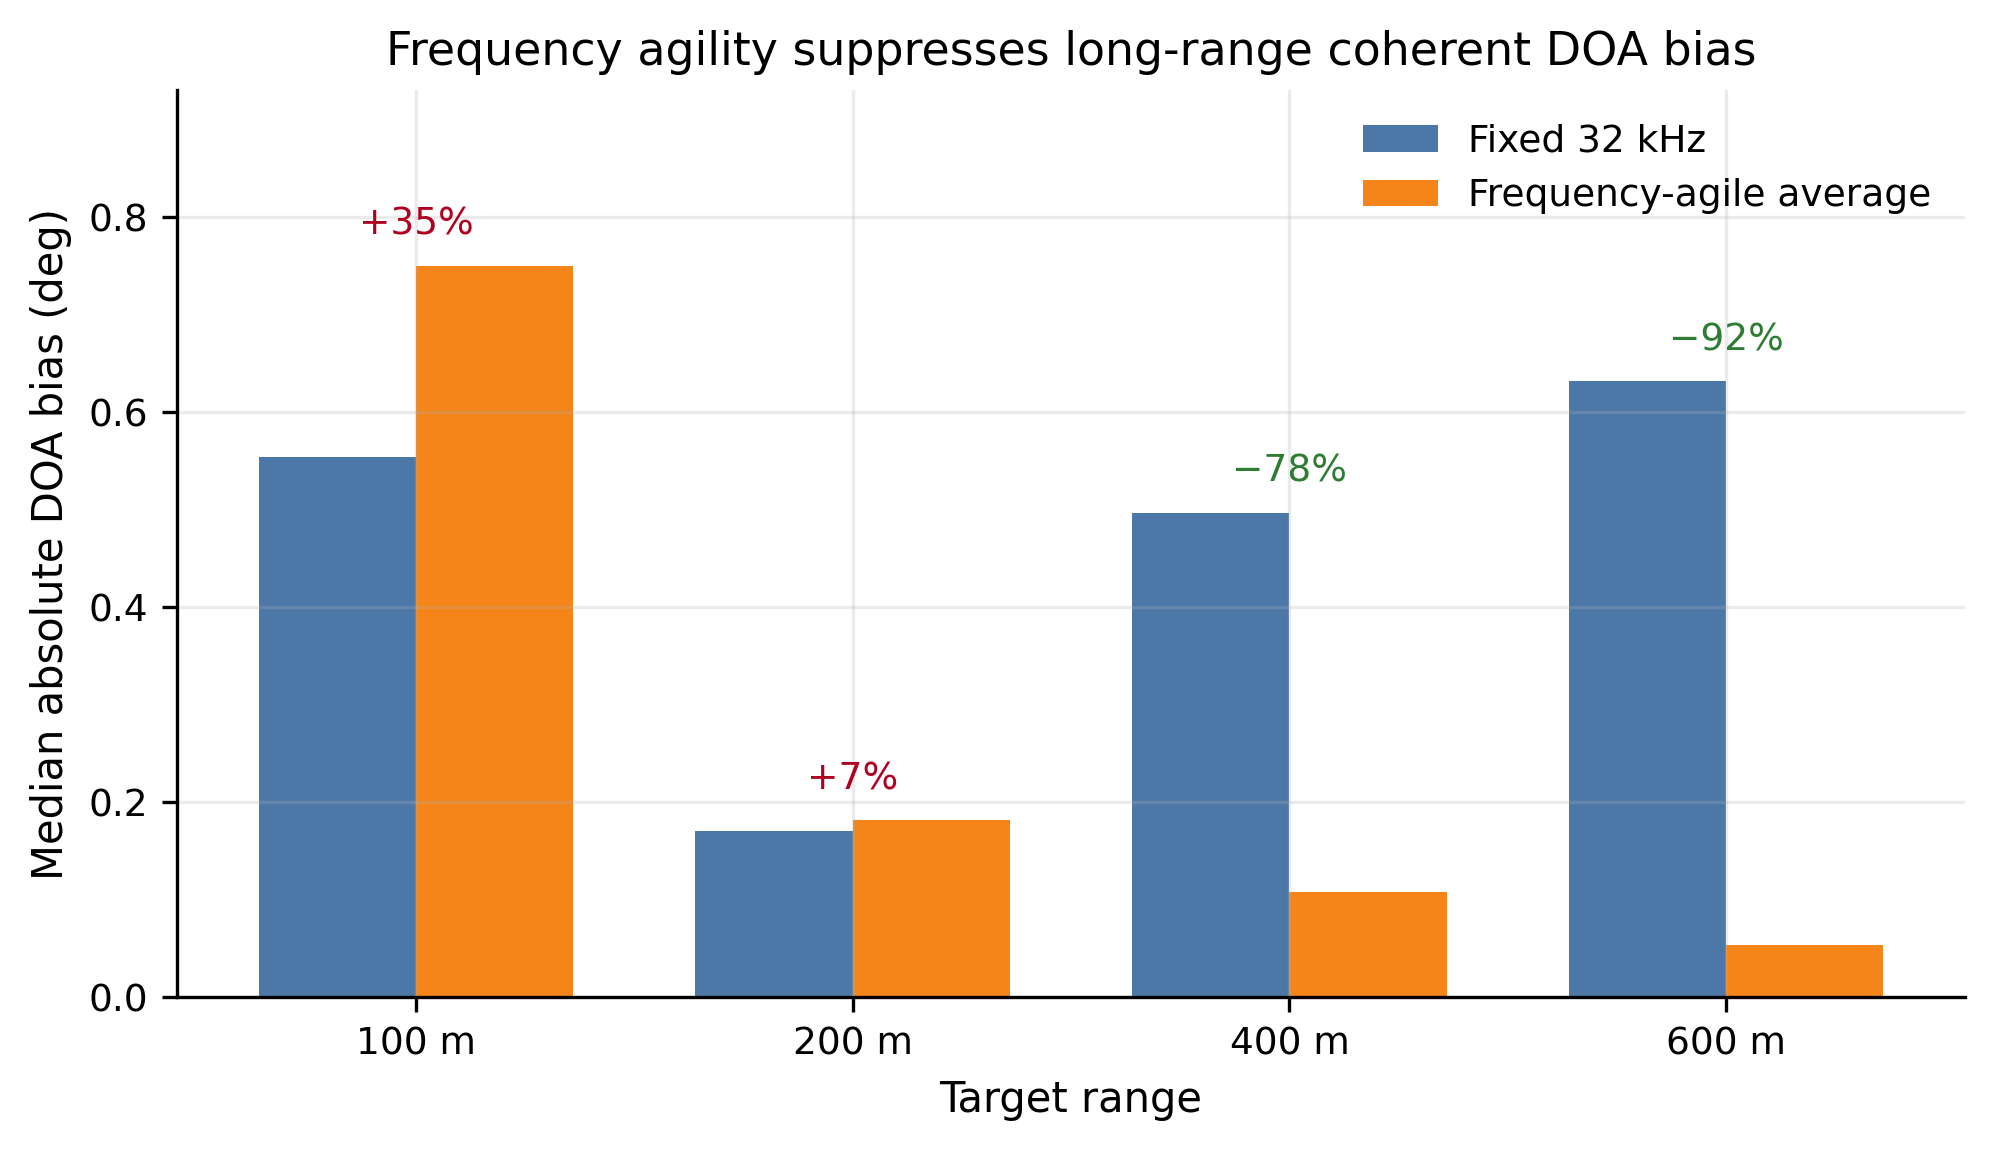
\includegraphics[width=\columnwidth]{fig2_frequency_agile_bias.png}
\caption{Carrier sensitivity of the long-range elevation-bias component. The fixed 32~kHz case
retains a larger median absolute bias at 600~m, while the 30--34~kHz carrier-agile average
strongly reduces the carrier-locked component. This supports the interpretation that the
post-gating residual contains a coherent frequency-dependent term.}
\label{fig:bias}
\end{figure}

\begin{figure}[!t]
\centering
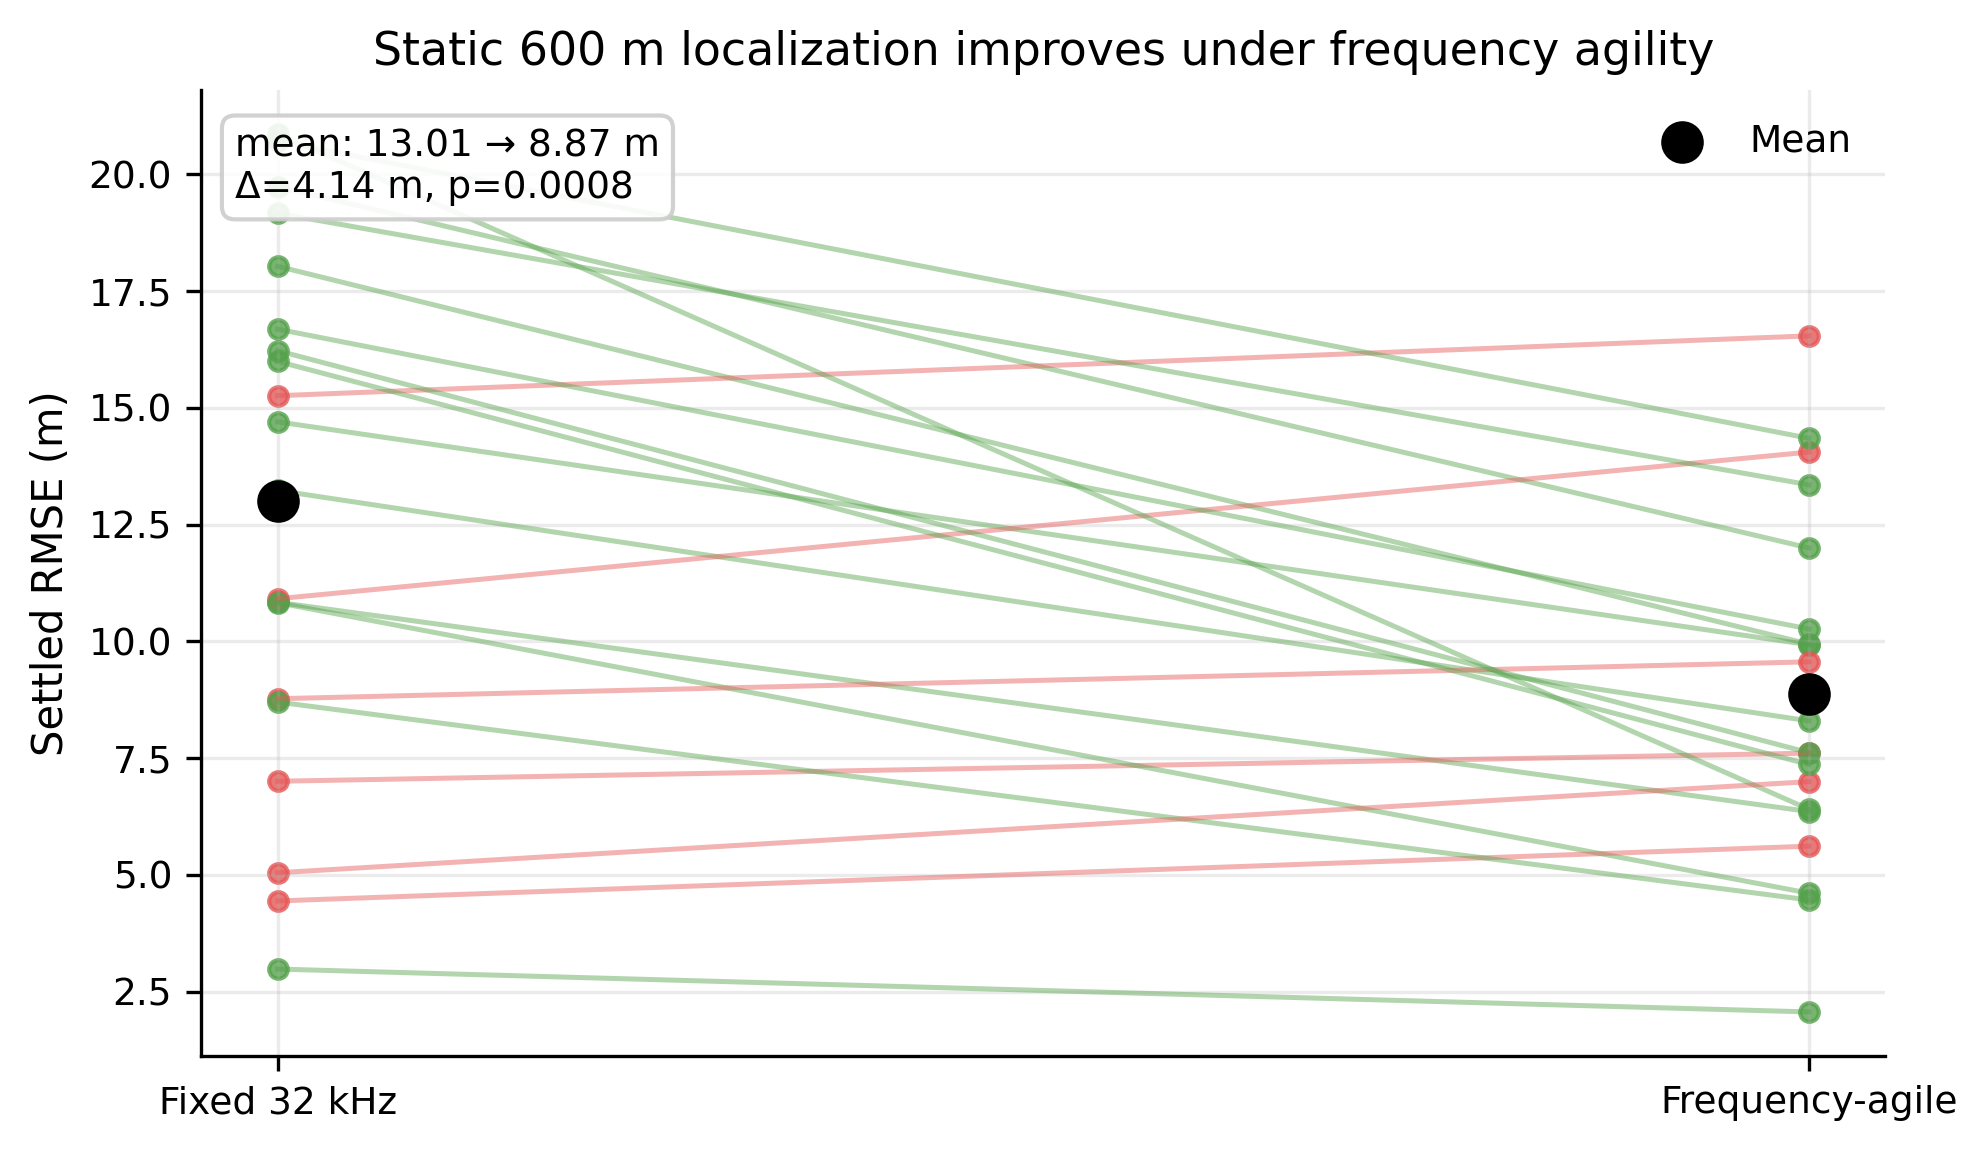
\includegraphics[width=\columnwidth]{fig3_static_600m_paired_rmse.png}
\caption{Independent static 600~m validation of the frozen carrier-agile schedule. Mean settled
RMSE decreased from 13.01~m under fixed 32~kHz transmission to 8.87~m under the 30--34~kHz
ping-to-ping schedule, corresponding to a $+4.14$~m paired improvement ($p=0.0008$).}
\label{fig:static}
\end{figure}

\begin{figure}[!t]
\centering
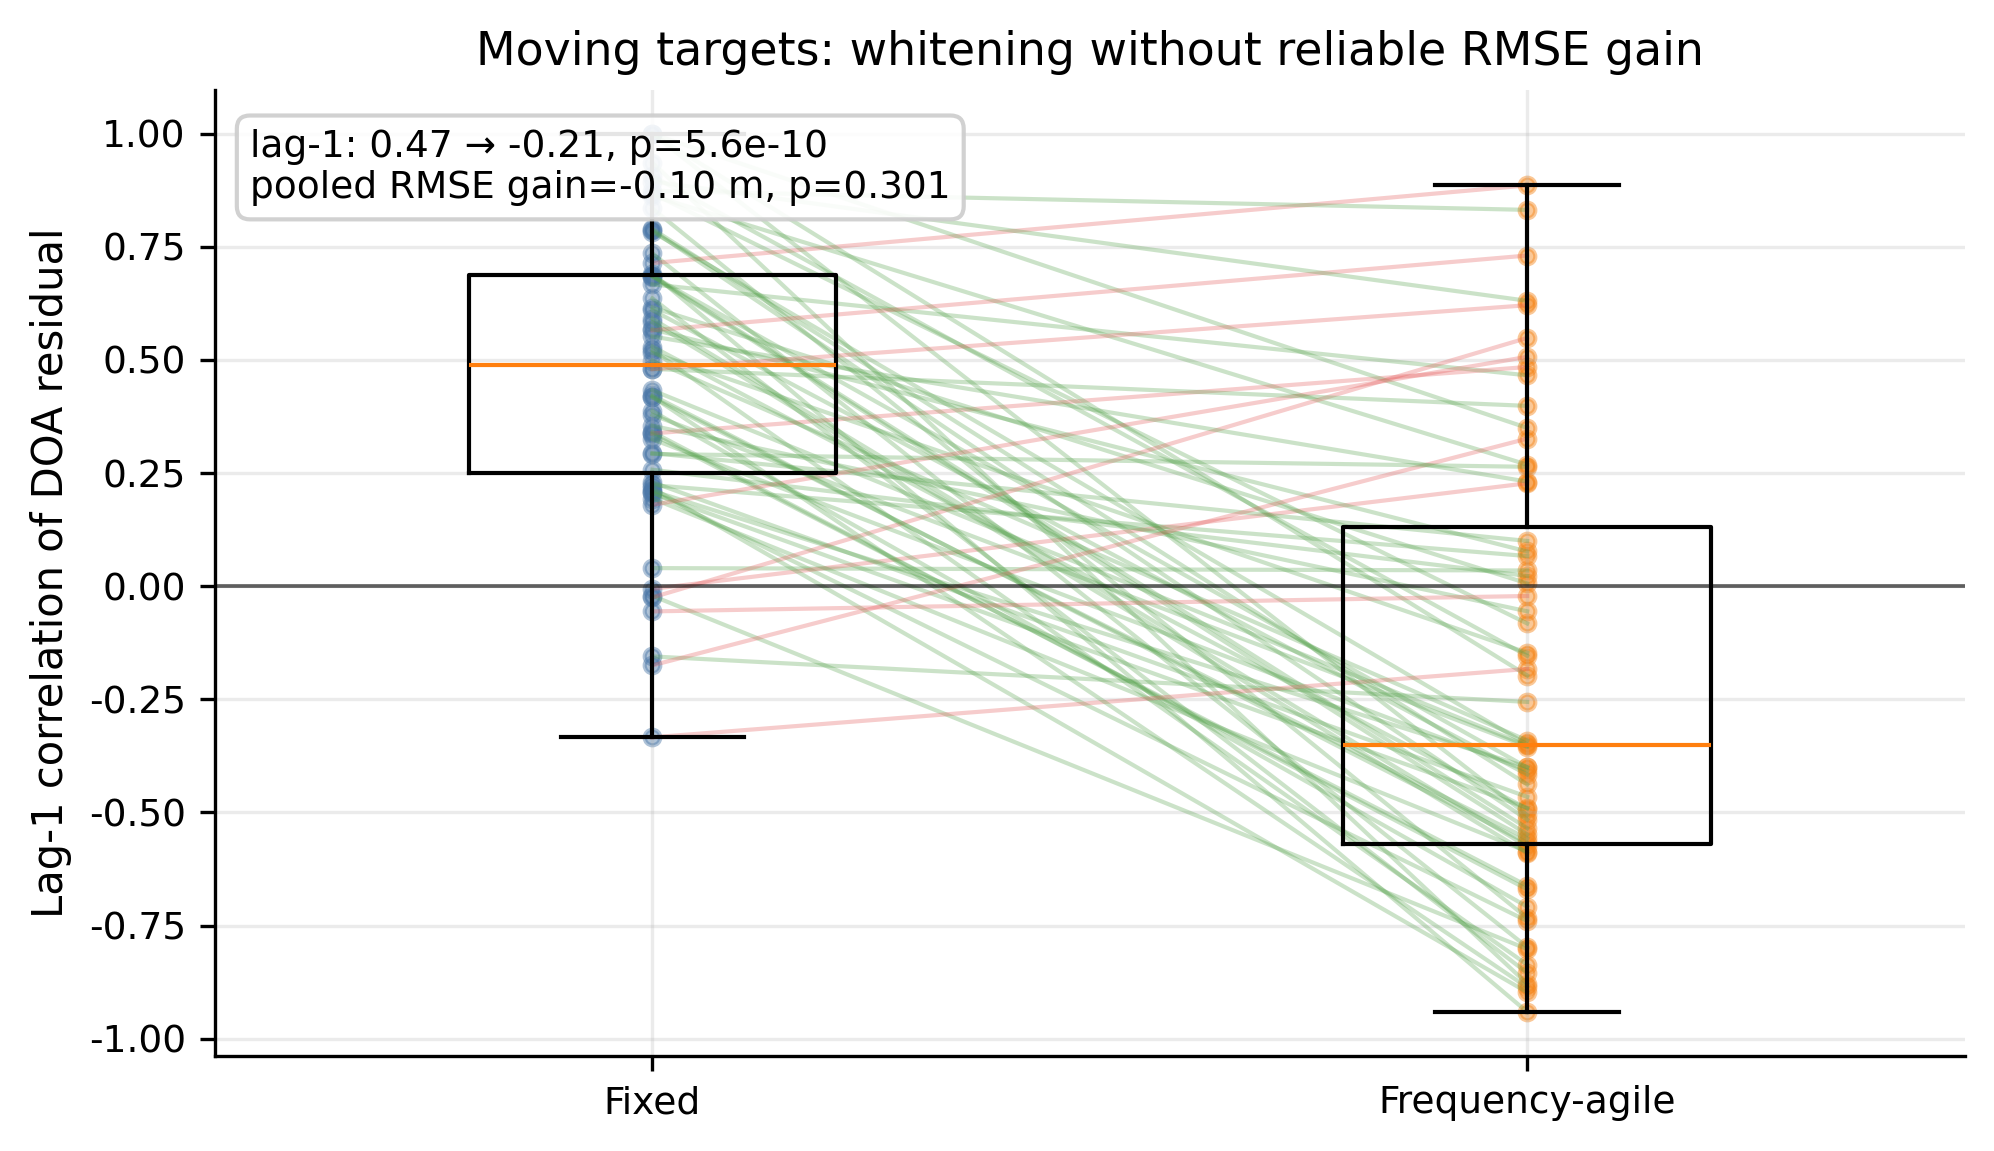
\includegraphics[width=\columnwidth]{fig4_moving_whitening_lag1.png}
\caption{Moving-target residual whitening and performance boundary. Carrier agility changed the
elevation residual lag-1 correlation from $+0.470$ to $-0.208$ ($p=5.56\times10^{-10}$), but the
pooled moving-target RMSE gain was not significant ($-0.10$~m, $p=0.301$). The figure supports a
mechanism claim, not a moving-target RMSE-improvement claim.}
\label{fig:moving}
\end{figure}

\begin{figure}[!t]
\centering
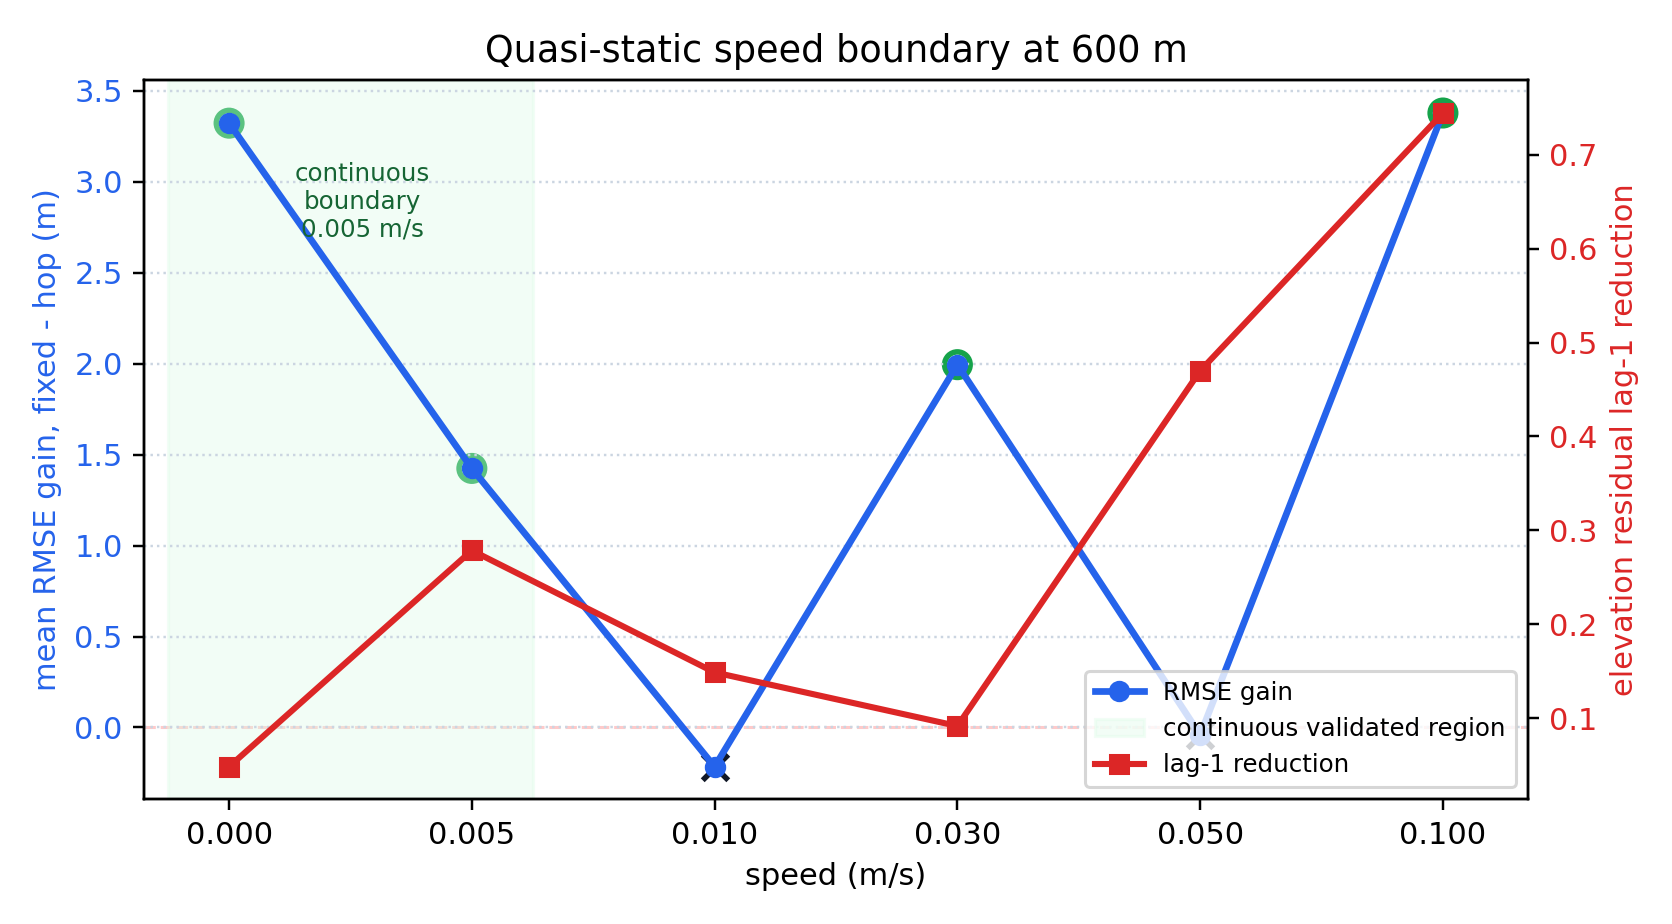
\includegraphics[width=\columnwidth]{fig5_quasi_static_speed_boundary.png}
\caption{Quasi-static speed sweep at 600~m. Static and 0.005~m/s drift were validated, whereas
0.010 and 0.050~m/s were not supported. Positive results at 0.030 and 0.100~m/s are treated as
geometry-dependent recoveries rather than a continuous speed boundary. The conservative continuous
boundary is 0.005~m/s under the present protocol.}
\label{fig:quasi}
\end{figure}

\begin{figure}[!t]
\centering
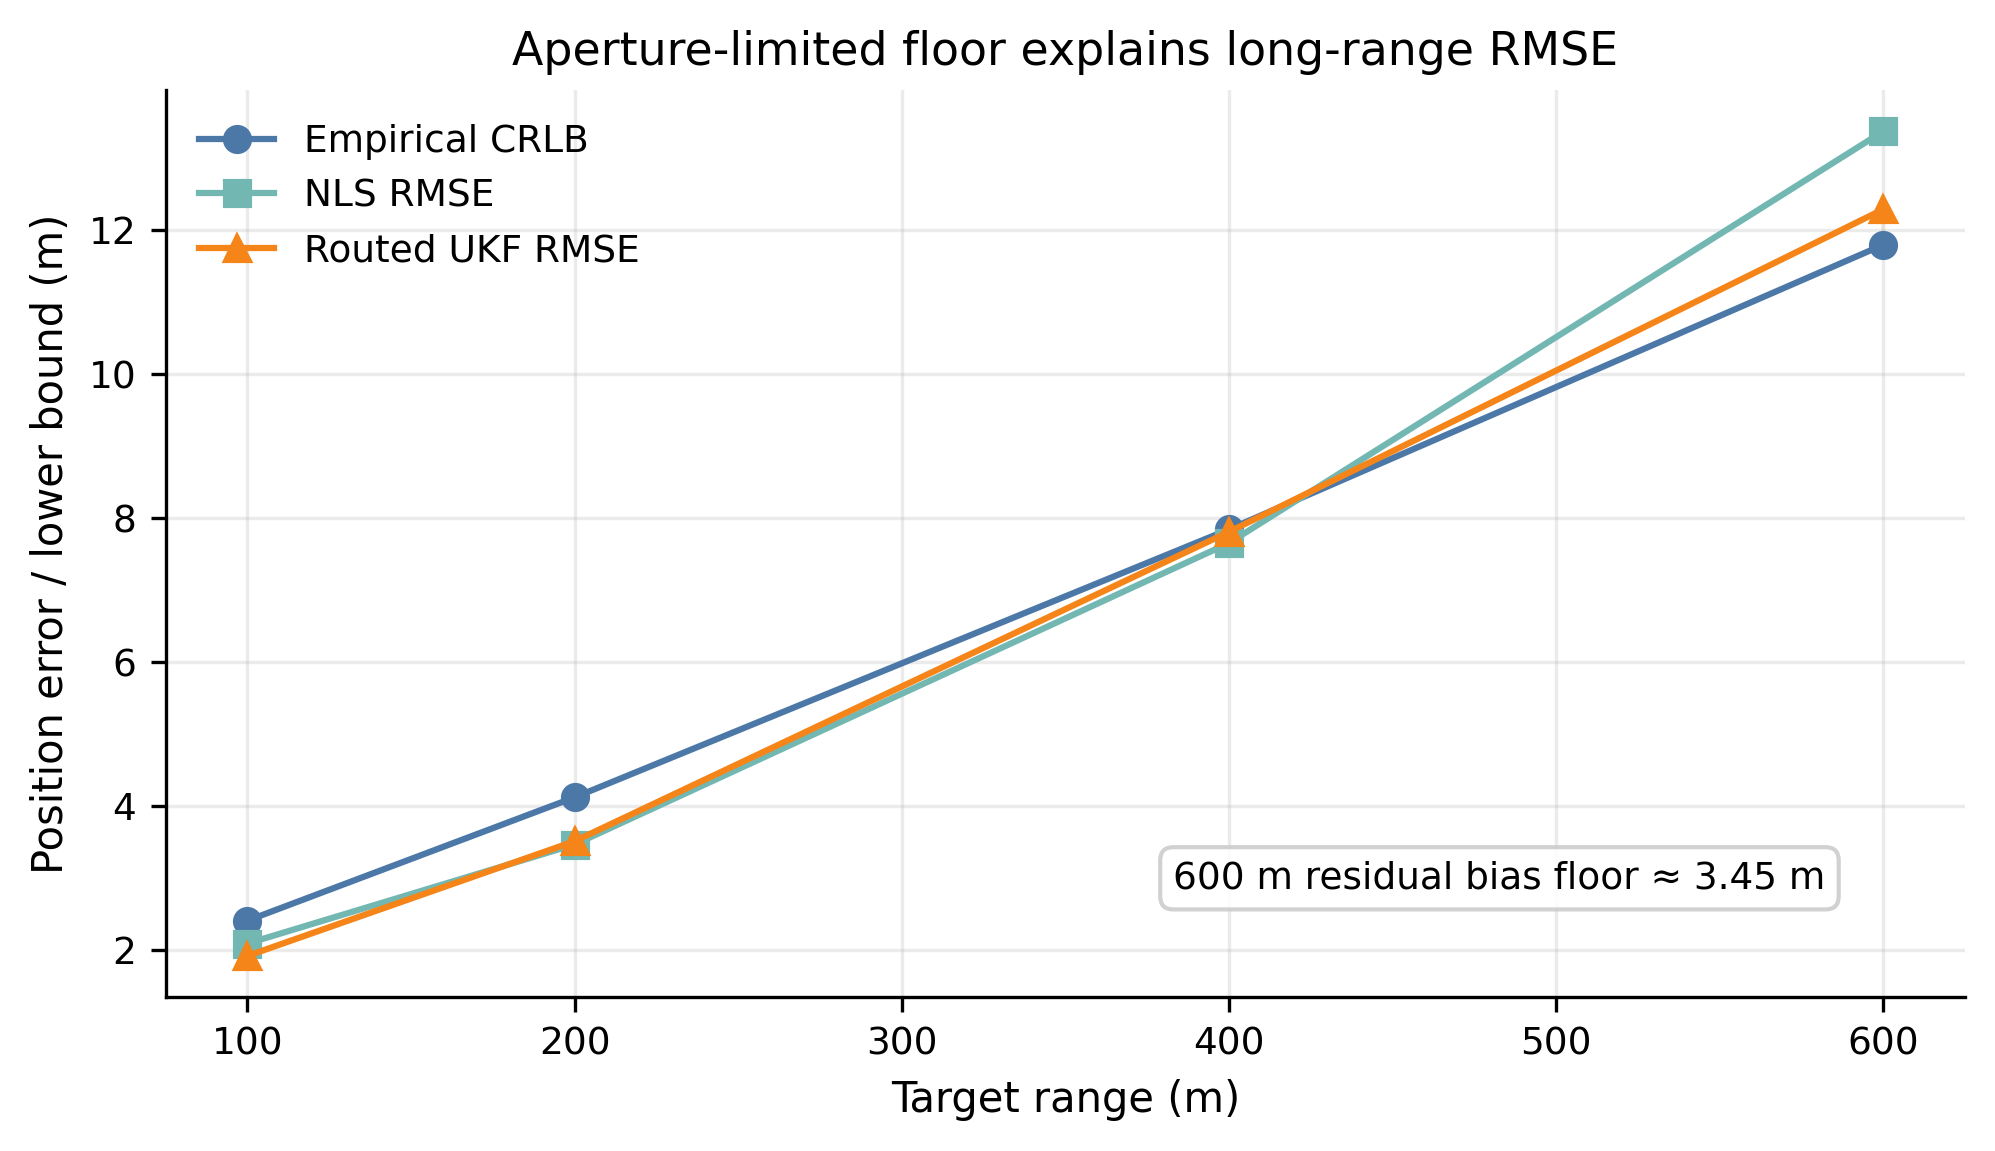
\includegraphics[width=\columnwidth]{fig6_crlb_floor.png}
\caption{Compact-aperture floor at long range. The 600~m empirical CRLB-scale reference is about
11.80~m, routed UKF is about 12.29~m, and NLS is about 13.38~m, showing that sub-meter long-range
performance is not expected under the present geometry and noise assumptions. Carrier agility
mitigates one coherent residual component; it does not remove the aperture/geometry floor.}
\label{fig:floor}
\end{figure}

\section*{Supplementary Materials}
The following supporting information should be supplied before submission: simulation scripts,
frozen carrier schedules, validation result JSON/CSV files, and figure-generation scripts for
Figs.~\ref{fig:concept}--\ref{fig:floor}. (Draft statement pending final data policy.)

\section*{Author Contributions}
Human-author decision required before submission. Do not submit this placeholder.

\section*{Funding}
Human-author decision required before submission. If there was no external funding, replace this
placeholder with the target journal's required no-funding statement.

\section*{Data Availability Statement}
The simulation outputs and analysis scripts supporting the reported results will be made available
through a public repository, archived release, supplementary material, or author-approved
access-on-request route. Before submission, replace this sentence with the exact URL, DOI, or
access policy selected by the authors.

\section*{Acknowledgments}
Human-author decision required before submission. Remove this section if the final target journal
allows omission and no acknowledgments are needed.

\section*{Conflicts of Interest}
Human-author decision required before submission. If there are no conflicts, replace this
placeholder with the target journal's required no-conflict statement.

\bibliographystyle{IEEEtran}
\bibliography{refs}

\end{document}
